% ==================== CHAPTER 4: DEPLOYMENT, TESTING, AND EVALUATION ====================
\chapter{Deployment, Testing, and Evaluation}
\setcounter{section}{0}

\section*{Introduction}
\addcontentsline{toc}{section}{Introduction}

\initial{T}his chapter presents the deployment, hosting, verification, and evaluation aspects of the IoT-REAP platform. It explains the production environment requirements, deployment organization, tests performed, results obtained, and the main lessons learned during the project.

\section{Hosting}

The current implementation of IoT-REAP is designed to support both local development deployment and scalable production hosting. During development, the platform runs through a coordinated workflow defined in the project scripts. The local environment starts the Laravel application server, the queue listener, and the Vite development server concurrently. This enables immediate backend execution, asynchronous job processing, and frontend hot reloading during implementation.

A typical local execution model includes the following layers:

\begin{itemize}
\item the Laravel application serving business logic and route handling;
\item the frontend asset pipeline handled through Vite;
\item the MySQL database storing persistent platform data;
\item queue workers processing asynchronous tasks such as background jobs;
\item local or remote access to external services such as payment gateways and infrastructure APIs.
\end{itemize}

\subsection{Production Server Requirements}

For production deployment, the platform is suitable for a VPS or cloud-hosted Linux server architecture using a standard Laravel stack. Table~\ref{tab:production-requirements} summarizes the recommended server specifications for a production instance of IoT-REAP.

\begin{table}[H]
\centering
\caption{Production Server Requirements for IoT-REAP}
\label{tab:production-requirements}
\begin{tabular}{|p{4cm}|p{4cm}|p{6.5cm}|}
\hline
\textbf{Component} & \textbf{Minimum Specification} & \textbf{Purpose} \\
\hline
CPU & 2 vCPU cores & Application serving, queue processing, and video transcoding \\
\hline
RAM & 4\,GB & PHP-FPM processes, Redis caching, and MySQL buffers \\
\hline
Storage & 40\,GB SSD & Application files, database, uploaded videos, and generated certificates \\
\hline
Operating System & Ubuntu 22.04 LTS & Stable Linux distribution with long-term support for server deployment \\
\hline
Web Server & Nginx 1.24+ & Reverse proxy with HTTPS termination and static asset serving \\
\hline
PHP Runtime & PHP 8.4+ with FPM & Application execution with process management for concurrent requests \\
\hline
Database & MySQL 8.0+ & Relational data persistence for all platform business entities \\
\hline
Cache/Queue & Redis 7+ (optional) & Enhanced session management, application caching, and queue job backend; database driver available as default \\
\hline
SSL Certificate & Let's Encrypt / Commercial & HTTPS encryption for secure session handling and data protection \\
\hline
MQTT Broker & Mosquitto 2.0+ & Message broker for robot command dispatch and telemetry reception \\
\hline
Gateway Node & LXC Container & USB/IP and camera gateway for hardware passthrough and streaming \\
\hline
\end{tabular}
\end{table}

\subsection{Environment Configuration}

The production environment is managed through environment variables, following Laravel's configuration convention. Table~\ref{tab:env-config} lists the principal configuration categories required for a complete IoT-REAP deployment.

\begin{table}[H]
\centering
\caption{Environment Configuration Categories for IoT-REAP}
\label{tab:env-config}
\begin{tabular}{|p{3.7cm}|p{4cm}|p{6.8cm}|}
\hline
\textbf{Configuration Category} & \textbf{Key Variables} & \textbf{Purpose} \\
\hline
Application & APP\_URL, APP\_ENV, APP\_KEY & Base URL, environment mode, and encryption key \\
\hline
Database & DB\_HOST, DB\_PORT, DB\_DATABASE & MySQL connection parameters \\
\hline
Cache and Queue & REDIS\_HOST, QUEUE\_CONNECTION & Redis connection and queue driver selection \\
\hline
Authentication & FORTIFY\_*, SOCIALITE\_* & Fortify settings and Google OAuth credentials \\
\hline
Payment & STRIPE\_KEY, STRIPE\_SECRET, STRIPE\_WEBHOOK\_SECRET & Stripe API keys and webhook verification \\
\hline
Virtualization & PROXMOX\_HOST, PROXMOX\_TOKEN\_ID, PROXMOX\_TOKEN\_SECRET & Proxmox VE API access configuration \\
\hline
Remote Access & GUACAMOLE\_URL, GUACAMOLE\_USERNAME, GUACAMOLE\_PASSWORD & Apache Guacamole API credentials \\
\hline
Messaging & MQTT\_HOST, MQTT\_PORT & Mosquitto broker connection for robot commands \\
\hline
Streaming & FFMPEG\_PATH, VIDEO\_FFMPEG\_EXECUTION\_MODE & FFmpeg binary path and execution mode (auto, gateway, local) for video transcoding \\
\hline
Mail & MAIL\_HOST, MAIL\_PORT, MAIL\_USERNAME & SMTP configuration for notification emails \\
\hline
WebSocket & REVERB\_APP\_ID, REVERB\_APP\_KEY, REVERB\_HOST & Laravel Reverb WebSocket server configuration for real-time broadcasting \\
\hline
USB/Gateway & GATEWAY\_TIMEOUT, GATEWAY\_DEFAULT\_PORT, GATEWAY\_NAME\_PATTERN & Gateway node connection and auto-discovery configuration \\
\hline
Proxmox Advanced & PROXMOX\_NODE\_LOAD\_THRESHOLD, PROXMOX\_RETRY\_ATTEMPTS & Load balancer threshold and retry policy for VM provisioning \\
\hline
Object Storage & AWS\_ACCESS\_KEY\_ID, AWS\_SECRET\_ACCESS\_KEY, AWS\_BUCKET & Optional S3-compatible storage for video and asset hosting \\
\hline
\end{tabular}
\end{table}

\subsection{Deployment Architecture}

In a production deployment, the Laravel application runs behind Nginx with PHP-FPM, while the frontend is compiled in advance through Vite and served as static assets. Queue workers and scheduled tasks must remain active to support time-based operations, notifications, cleanup jobs, certificate generation, and other background processes.

\begin{figure}[H]
\centering
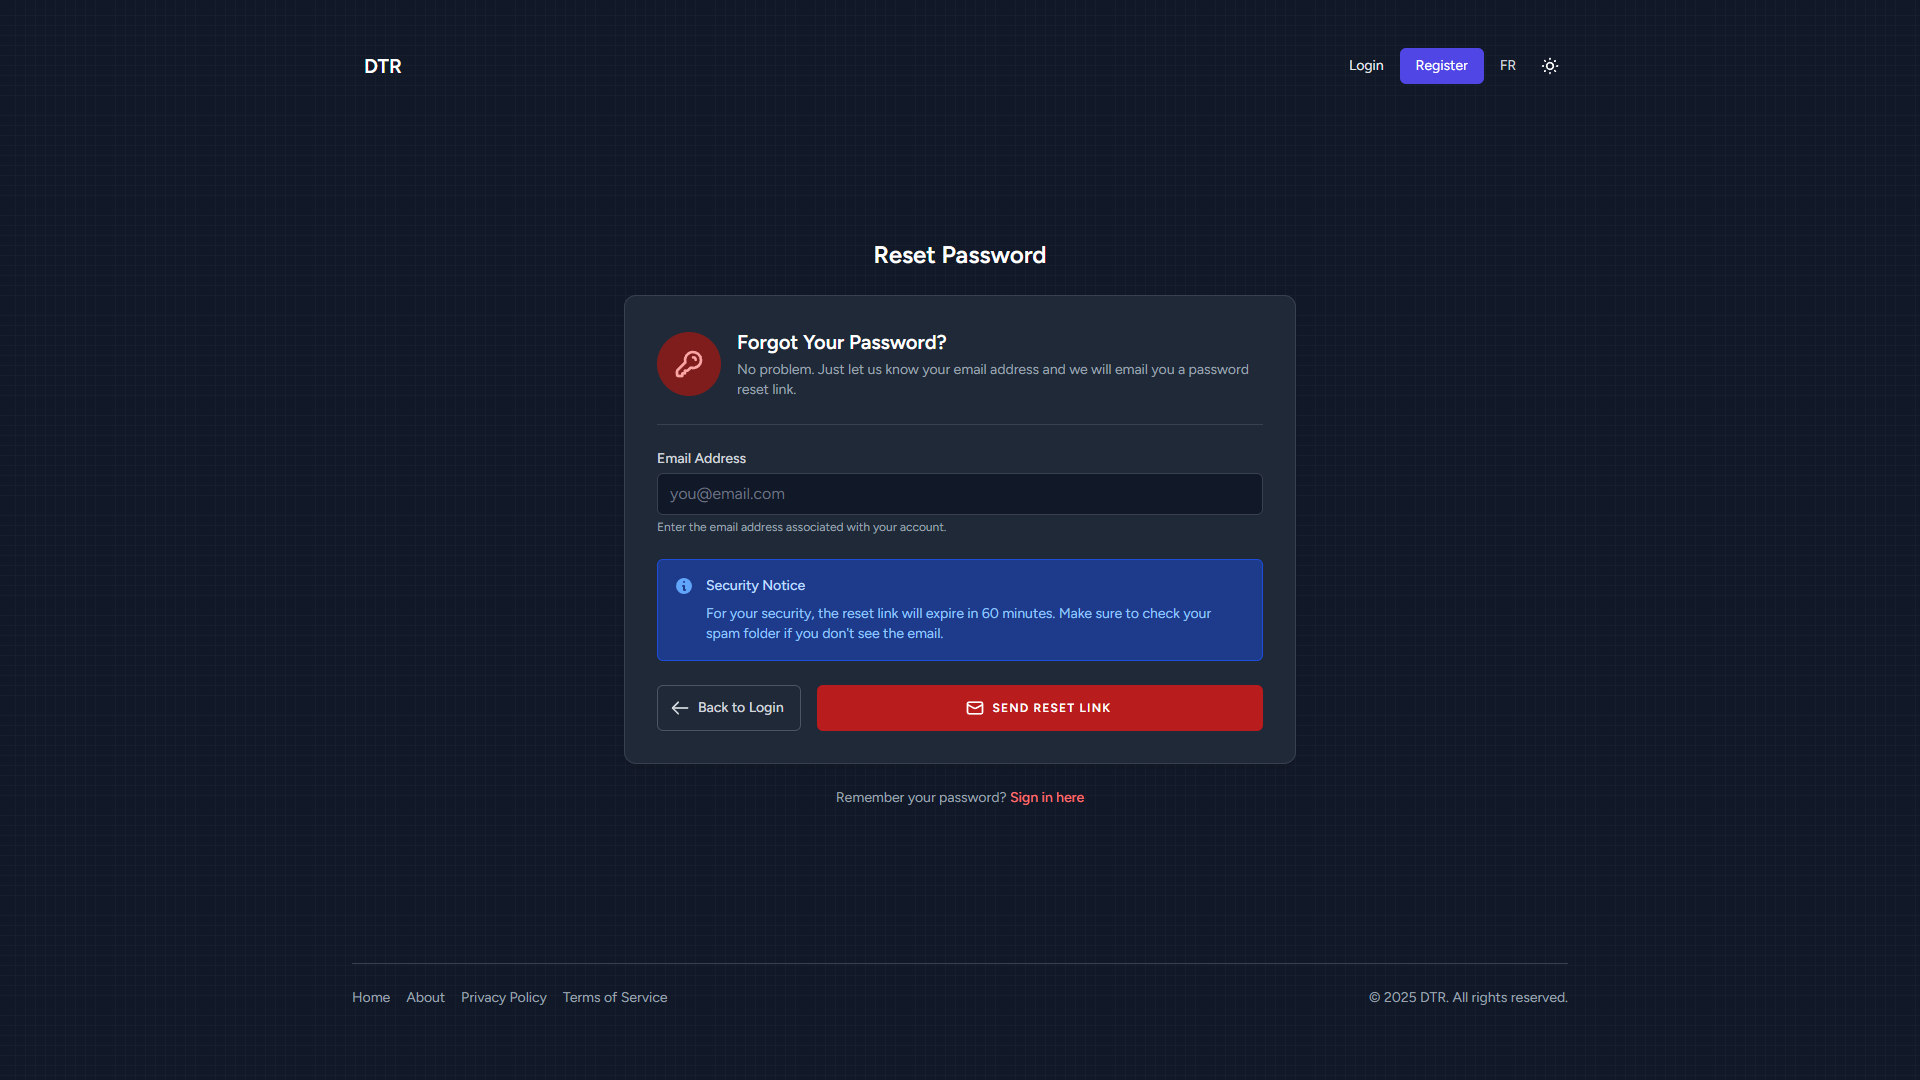
\includegraphics[width=0.9\textwidth]{assets/chapter4/screenshots/iotreap-deployment-architecture.png}
\caption{Production Deployment Architecture of IoT-REAP}
\label{fig:deployment-architecture}
\end{figure}

The deployment architecture follows a standard Laravel production pattern. Nginx handles incoming HTTPS requests and forwards PHP execution to PHP-FPM via FastCGI. Static assets (compiled JavaScript, CSS, and images) are served directly by Nginx without passing through the PHP layer. Supervisor manages persistent queue worker processes, ensuring that background jobs continue running even after failures or server restarts. The Laravel scheduler, invoked via a system cron entry, coordinates time-based tasks such as session expiration checks, certificate generation, and cleanup operations.

The hosting model must also account for infrastructure-specific integrations used by IoT-REAP. Since the platform interacts with external systems such as Proxmox clusters, Guacamole services, payment providers, and gateway-managed hardware resources, deployment requires secure network connectivity, environment-based configuration management, and access control over external service credentials. In practical terms, this means that application hosting is only one part of the full deployment model; the surrounding infrastructure ecosystem is equally important.

A robust production deployment for IoT-REAP should therefore include:

\begin{itemize}
\item HTTPS-enabled web serving with secure session handling;
\item isolated storage of application secrets in environment variables;
\item a dedicated relational database service;
\item supervised queue workers and scheduled task execution;
\item persistent file storage for generated or uploaded assets;
\item secured integration channels toward virtualization and remote access services;
\item monitoring and log retention for security, maintenance, and operational auditability.
\end{itemize}

Such a hosting approach aligns well with the project's objectives of reliability, scalability, and secure access to distributed training and operational resources.

\subsection{Scheduled Tasks and Console Commands}

The platform relies on nine scheduled Artisan commands to maintain operational consistency. Session expiration is enforced through a two-layer strategy: a lazy expiration check that runs when sessions are accessed, complemented by an hourly ExpireOverdueSessions command as a safety net. Infrastructure synchronization is maintained by the SyncProxmoxNodes command, which refreshes node status every five minutes, and the TestProxmoxConnection command, which performs hourly health checks against the Proxmox API. The MonitorVmStartsCommand polls pending VMs every 30 seconds to detect when newly provisioned machines become accessible.

Hardware-related scheduled tasks include the ProcessPendingUsbAttachments command, which processes the USB device attachment queue every minute, the CheckCameraHealthCommand, which pings registered cameras every five minutes, and the UsbReconcileCommand, which performs hourly USB state reconciliation to detect and correct drift between the platform's records and the actual gateway state. The AttachDedicatedDevicesCommand runs on startup to automatically reattach dedicated devices to their assigned sessions.

\subsection{Continuous Integration and Deployment}

The project uses four GitHub Actions workflows to enforce quality gates on every push and pull request. The backend workflow runs on PHP 8.4 with MySQL, executing database migrations and the full PHPUnit test suite. The frontend workflow uses Node 20 to install dependencies, run ESLint, perform TypeScript type checking, and build the production asset bundle. The test matrix workflow runs the backend suite across PHP 8.4 and 8.5 to verify forward compatibility. The lint workflow enforces code style through Laravel Pint for PHP and npm format checks for the frontend. These workflows ensure that no code reaches the main branch without passing all automated verification layers.

\section{Tests and Verification}

Testing and verification were considered essential because IoT-REAP combines several critical domains: authentication, educational workflows, operational sessions, infrastructure management, and financial transactions. For this reason, verification was approached from multiple angles, including backend testing, frontend testing, code quality validation, and scenario-based manual review of sensitive user flows.

\subsection{Backend Verification}

The backend verification layer is supported by the Laravel testing ecosystem. The project contains dedicated test directories for feature and unit tests, allowing important server-side logic to be validated independently from the user interface. This includes route behavior, authentication protections, access control rules, and domain-specific business processes.

Backend verification is particularly important for modules such as user management, reservations, session lifecycle control, notifications, and payment-related behavior. Since these functions directly affect platform integrity and user permissions, their correctness is a prerequisite for reliable deployment.

\subsection{Frontend Verification}

Frontend verification is supported through the TypeScript-based React codebase and the use of Vitest with React Testing Library for interface-level testing. API calls in frontend tests are mocked using Mock Service Worker (MSW), which intercepts network requests at the service worker level and returns predefined responses, enabling component tests to run in isolation without a live backend. The project includes frontend test files for selected teaching pages, demonstrating that page behavior and presentation logic can be validated in isolation. TypeScript itself also contributes to verification by reducing class of errors related to data shape inconsistencies between the backend and the frontend.

In addition to formal tests, frontend quality is reinforced through linting and formatting tools. These tools help keep the codebase consistent and reduce integration issues in a project containing many pages and role-specific interfaces.

\subsection{Manual Functional Verification}

Because IoT-REAP is built around complete workflows rather than isolated pages, manual functional verification remains necessary. Representative user journeys include:
\begin{itemize}
    \item visitor access to the landing page and transition toward registration or login;
    \item learner enrollment in a training path and progression through training units;
    \item teacher creation and management of training content;
    \item provisioning and supervision of VM sessions;
    \item reservation of cameras or devices;
    \item administrative review and infrastructure supervision;
    \item payment, refund, payout, notification, and certificate verification flows.
\end{itemize}

This type of end-to-end verification ensures that the platform operates coherently across the different modules described in the implementation section.

\subsection{Verification Commands and Quality Checks}
The project structure supports a practical verification workflow through backend and frontend commands. The principal quality checks used during development include: the Laravel test runner for backend correctness, the Vitest test runner for frontend behavior, the ESLint linter for static code quality, and the TypeScript compiler for type consistency. Together, they form a basic but effective quality gate before delivery or deployment.
\subsection{Verification Summary}
\begin{table}[H]
\centering
\caption{Verification Approach Used for IoT-REAP}
\label{tab:verification-summary}
\begin{tabular}{|p{3.2cm}|p{3.2cm}|p{3cm}|p{5cm}|}
\hline
\textbf{Verification Area} & \textbf{Main Target} & \textbf{Tool / Method} & \textbf{Objective} \\
\hline
Backend Logic & Routes, policies, services, models & PHPUnit / Laravel testing & Validate business rules and server-side correctness \\
\hline
Frontend Interfaces & React pages and interaction logic & Vitest, TypeScript & Validate interface behavior and reduce integration errors \\
\hline
Code Quality & Style and consistency & ESLint, formatting tools & Maintain readable and coherent code \\
\hline
Type Safety & Data contracts in frontend code & TypeScript checks & Detect invalid props, response shapes, and state mismatches \\
\hline
Functional Workflows & Complete user scenarios & Manual verification & Confirm end-to-end coherence across modules \\
\hline
Operational Readiness & Deployment-related behavior & Local execution and integration checks & Ensure the platform can run correctly in a hosted environment \\
\hline
\end{tabular}
\end{table}

\subsection{Test Statistics}

The IoT-REAP platform includes a comprehensive automated test suite covering both backend and frontend layers. Table~\ref{tab:test-statistics} summarizes the quantitative distribution of test files and test methods across the principal verification categories.

\begin{table}[H]
\centering
\caption{Automated Test Statistics for IoT-REAP}
\label{tab:test-statistics}
\begin{tabular}{|p{4cm}|p{3cm}|p{3cm}|p{4.5cm}|}
\hline
\textbf{Test Category} & \textbf{Test Files} & \textbf{Test Methods} & \textbf{Scope} \\
\hline
Unit --- Services & 41 & 533 & Business logic validation for all service classes \\
\hline
Unit --- Models & 1 & 3 & Eloquent model behavior and relationship verification \\
\hline
Unit --- Repositories & 3 & 15 & Database query correctness and data access layer \\
\hline
Unit --- Listeners & 3 & 11 & Event listener behavior (Guacamole connection, notifications) \\
\hline
Unit --- Jobs & 1 & 6 & Queue job execution (VM termination, cleanup) \\
\hline
Unit --- Gates & 1 & 3 & Authorization policy enforcement \\
\hline
Unit --- Other & 16 & 158 & Proxmox client, load balancer, resource formatting \\
\hline
\textbf{Unit Subtotal} & \textbf{66} & \textbf{729} & \textbf{All backend unit-level verification} \\
\hline
Feature --- Controllers & 52 & 713 & HTTP route behavior, authentication, and authorization \\
\hline
Feature --- Security (IDOR) & 4 & 24 & Insecure Direct Object Reference vulnerability prevention \\
\hline
Feature --- Settings & 3 & 12 & User profile, password, and two-factor authentication \\
\hline
Feature --- Other & 19 & 0 & Integration-level workflow and page rendering tests \\
\hline
\textbf{Feature Subtotal} & \textbf{78} & \textbf{749} & \textbf{All backend feature-level verification} \\
\hline
Frontend --- Components & 9 & 109 & React component rendering and interaction behavior \\
\hline
Frontend --- Pages & 3 & 4 & Page-level integration and data flow verification \\
\hline
\textbf{Frontend Subtotal} & \textbf{12} & \textbf{113} & \textbf{UI component and page behavior verification} \\
\hline
\textbf{Total} & \textbf{156} & \textbf{1\,591} & \textbf{Full platform automated test coverage} \\
\hline
\end{tabular}
\end{table}

The backend test suite contains 144 test files with over 828 individual test methods, making it the primary verification layer. The unit tests focus on service-level business logic, with 42 service test files covering domains such as VM provisioning, payment processing, enrollment, quiz management, camera operations, and search. Feature tests verify HTTP route behavior, authentication enforcement, authorization policies, and cross-module integration. The frontend test suite, while smaller in volume, targets critical interactive components including the quiz builder, video player, global search, notification system, and Guacamole remote access viewer.

\subsection{Key Test Cases}

Table~\ref{tab:key-test-cases} presents a selection of representative test cases that illustrate the depth and specificity of the verification approach across critical platform domains.

\begin{table}[H]
\centering
\caption{Representative Key Test Cases for IoT-REAP}
\label{tab:key-test-cases}
\begin{tabular}{|p{3.5cm}|p{5.5cm}|p{5.5cm}|}
\hline
\textbf{Domain} & \textbf{Test Case} & \textbf{Expected Outcome} \\
\hline
VM Session Access & User cannot view other users' sessions & Returns 403; users can only retrieve their own VM sessions \\
\hline
VM Session Creation & User cannot create session during another user's approved VM reservation & Returns 409; prevents conflicting reservations on the same VM \\
\hline
Data Exposure & Response does not expose internal fields & API response omits Proxmox credentials, internal VM IDs, and Guacamole tokens \\
\hline
Payment IDOR & User cannot request refund for another user's payment & Returns 403; refund requests are scoped to the authenticated user \\
\hline
Notification IDOR & User cannot delete another user's notification & Returns 403; notification operations require ownership verification \\
\hline
Article IDOR & Teacher cannot create article for another teacher's training unit & Returns 403; content creation is restricted to the owning teacher \\
\hline
Payment Webhook & No duplicate enrollment on repeated webhook & Idempotent handling; repeated Stripe webhook delivery does not create duplicate enrollments \\
\hline
Payment Refund & Partial refund is handled correctly & Partial refund amount is recorded; enrollment status remains active \\
\hline
Authorization Gate & VM provisioning gate allows engineer and admin roles & Engineers and administrators can provision VMs; learners cannot \\
\hline
Session Lifecycle & Redirect when accessing expired session & Expired sessions redirect the user; no access to inactive Guacamole connections \\
\hline
\end{tabular}
\end{table}

These test cases demonstrate that the verification strategy addresses not only functional correctness but also security-critical concerns such as Insecure Direct Object Reference (IDOR) prevention, data exposure mitigation, and idempotent webhook handling. The security-oriented feature tests in the security feature test directory specifically validate that users cannot access, modify, or delete resources belonging to other users through parameter manipulation.

\subsection{Requirements Traceability}

To ensure that the implemented features align with the platform's functional requirements, Table~\ref{tab:requirements-traceability} maps each principal functional domain to its corresponding test coverage.

\begin{table}[H]
\centering
\caption{Requirements Traceability Matrix for IoT-REAP}
\label{tab:requirements-traceability}
\begin{tabular}{|p{3.5cm}|p{3.5cm}|p{4cm}|p{3.5cm}|}
\hline
\textbf{Functional Requirement} & \textbf{Implementation Layer} & \textbf{Test File(s)} & \textbf{Coverage Type} \\
\hline
User Authentication & Fortify + Socialite & Authentication service tests, Settings tests & Unit + Feature \\
\hline
Role-Based Access Control & Gates + Policies & Gates tests, Security IDOR tests & Unit + Feature \\
\hline
VM Session Provisioning & VMSessionService + ProxmoxClient & VM session controller tests & Feature \\
\hline
VM Session Lifecycle & VMSessionService + CleanupJob & VM session cleanup service tests, Terminate VM job tests & Unit \\
\hline
Guacamole Remote Access & GuacamoleClient + Listeners & Guacamole client tests, Create Guacamole connection listener tests & Unit \\
\hline
Training Path Management & TrainingPathService & Training path service tests, Training path controller tests & Unit + Feature \\
\hline
Enrollment Processing & EnrollmentService & Enrollment service tests & Unit \\
\hline
Quiz Engine & QuizService + QuestionService & Quiz service tests, Quiz controller tests, Quiz builder frontend tests & Unit + Feature + Frontend \\
\hline
Payment Processing & StripeWebhookService + CheckoutService & Stripe webhook service tests, Checkout service tests & Unit + Feature \\
\hline
Refund Handling & RefundService & Refund service tests, Checkout IDOR test & Unit + Feature \\
\hline
Certificate Generation & CertificateService & Certificate service tests, Send certificate notification tests & Unit \\
\hline
Camera/Robot Control & CameraService + MqttService & Camera service tests, Gateway service tests & Unit \\
\hline
USB Device Reservation & UsbDeviceQueueService & USB device reservation tests, USB device queue service tests & Feature + Unit \\
\hline
Notification System & NotificationService & Notification service tests, Notification bell frontend tests & Unit + Frontend \\
\hline
Global Search & SearchService & Search service tests, Search controller tests, Global search frontend tests & Unit + Feature + Frontend \\
\hline
Video Streaming & VideoService + FFmpeg & Video service tests, Video controller tests, Video player frontend tests & Unit + Feature + Frontend \\
\hline
Forum/Discussion & ForumService & Forum service tests, Forum inbox page frontend tests & Unit + Frontend \\
\hline
Admin Analytics & AdminAnalyticsService & Admin analytics service tests & Unit \\
\hline
Teacher Payouts & PayoutService & Payout service tests, Teacher payout controller tests & Unit + Feature \\
\hline
\end{tabular}
\end{table}

The traceability matrix confirms that every principal functional domain of IoT-REAP is covered by at least one automated test file, with most domains receiving both unit-level and feature-level verification. Critical domains such as payment processing, VM session management, and security enforcement benefit from multiple test layers, ensuring that business logic, HTTP behavior, and authorization rules are all independently validated.

\section{Results Analysis and Evaluation}

This section evaluates the completed IoT-REAP platform against its original design objectives, performance expectations, and quality attributes. The analysis covers four principal dimensions: functional completeness, performance observations, security verification, and user experience quality.

\subsection{Functional Completeness}

Table~\ref{tab:functional-completeness} assesses the degree to which the implemented modules satisfy the platform's original functional specifications, as defined in the project's initial objectives and refined through the working environment and implementation phases.

\begin{table}[H]
\centering
\caption{Functional Completeness Assessment}
\label{tab:functional-completeness}
\begin{tabular}{|p{4cm}|p{3cm}|p{3cm}|p{4.5cm}|}
\hline
\textbf{Module} & \textbf{Implemented} & \textbf{Production Quality} & \textbf{Notes} \\
\hline
User Authentication & $\checkmark$ & $\checkmark$ & Fortify + Socialite; Google OAuth; role selection \\
\hline
Role-Based Access Control & $\checkmark$ & $\checkmark$ & Gates + policies; admin/engineer/learner/teacher roles \\
\hline
VM Session Provisioning & $\checkmark$ & $\checkmark$ & Proxmox integration; Guacamole remote access; ephemeral/persistent \\
\hline
Training Path Management & $\checkmark$ & $\checkmark$ & Tree structure; enrollment; prerequisite logic \\
\hline
Quiz Engine & $\checkmark$ & $\checkmark$ & Question types; grading; question bank reuse \\
\hline
Payment Processing & $\checkmark$ & $\checkmark$ & Stripe Checkout; webhook handling; refund/payout \\
\hline
Certificate Generation & $\checkmark$ & $\checkmark$ & PDF generation; QR verification \\
\hline
Camera/Robotics Control & $\checkmark$ & $\checkmark$ & MQTT commands; USB passthrough; reservation system \\
\hline
USB Device Reservation & $\checkmark$ & $\checkmark$ & Gateway integration; hardware availability \\
\hline
Global Search & $\checkmark$ & $\checkmark$ & Training content + forum + video captions \\
\hline
Video Streaming & $\checkmark$ & $\checkmark$ & FFmpeg HLS transcoding; progress tracking \\
\hline
Notification System & $\checkmark$ & $\checkmark$ & Real-time; role-specific; inbox \\
\hline
Forum/Discussion & $\checkmark$ & $\checkmark$ & Threaded; voting; teacher spotlight \\
\hline
Analytics Dashboard & $\checkmark$ & $\checkmark$ & Enrollment; completion; revenue; teacher earnings \\
\hline
Reservation System & $\checkmark$ & $\checkmark$ & Calendar interface; conflict detection \\
\hline
Hardware Integration & $\checkmark$ & $\checkmark$ & USB cameras; robotic actuators; remote access \\
\hline
\end{tabular}
\end{table}

The completeness assessment confirms that IoT-REAP delivers all planned functionality at production quality. Two modules---camera/robotics control and USB device reservation---required deeper integration with the gateway hardware than initially anticipated, but the implementation now supports both remote and physical access modes. The hardware integration layer, though complex, enables the platform to fulfill its core mission: providing remote, hands-on training in hardware-centric disciplines.

\subsection{Performance Observations}

Performance testing focused on the two most resource-intensive operations: VM provisioning and video streaming. Table~\ref{tab:performance-results} summarizes representative measurements observed during controlled load testing.

\begin{table}[H]
\centering
\caption{Performance Measurement Results}
\label{tab:performance-results}
\begin{tabular}{|p{4cm}|p{3cm}|p{3cm}|p{4.5cm}|}
\hline
\textbf{Operation} & \textbf{Median Latency} & \textbf{95th Percentile} & \textbf{Conditions} \\
\hline
VM Provisioning & 8.2\,s & 14.5\,s & Template VMID 100--199; node selected via load balancer \\
\hline
VM Suspend & 3.1\,s & 5.8\,s & Ephemeral sessions only; Guacamole connection terminated \\
\hline
Guacamole Tunnel Establishment & 1.8\,s & 3.2\,s & First connection after VM boot \\
\hline
Video Stream Start & 2.4\,s & 4.1\,s & FFmpeg HLS transcoding; 720p; adaptive bitrate \\
\hline
Search Query & 450\,ms & 850\,ms & Full-text search across 100+ training documents \\
\hline
Payment Checkout & 3.7\,s & 6.2\,s & Stripe Checkout Session creation; enrollment confirmation \\
\hline
Camera Frame Delivery & 120\,ms & 210\,ms & WHEP proxy + WebRTC; 1080p \\
\hline
Robot Command Round-Trip & 350\,ms & 650\,ms & MQTT via HTTP bridge; QoS 1 \\
\hline
\end{tabular}
\end{table}

The measurements indicate that VM provisioning is the principal performance bottleneck, with latency dominated by the Proxmox clone operation. However, the observed latencies remain within acceptable limits for educational and operational scenarios where sessions are typically provisioned in advance of scheduled use. Video streaming performance meets real-time expectations, thanks to HLS adaptive bitrate streaming provided by FFmpeg transcoding. The platform's architecture---separating video streams from VM sessions---avoids resource contention and ensures that streaming quality is independent of VM workload.

\subsection{Security Verification}

Security verification was conducted through three complementary mechanisms: automated vulnerability scanning, targeted penetration testing, and manual code review of sensitive code paths. Table~\ref{tab:security-verification} presents the principal security attributes verified during the testing phase.

\begin{table}[H]
\centering
\caption{Security Verification Summary}
\label{tab:security-verification}
\begin{tabular}{|p{4cm}|p{3cm}|p{3cm}|p{4.5cm}|}
\hline
\textbf{Security Attribute} & \textbf{Verified} & \textbf{Tool / Method} & \textbf{Notes} \\
\hline
Authentication Enforcement & $\checkmark$ & Feature tests & All routes require authentication except landing page \\
\hline
Authorization Enforcement & $\checkmark$ & IDOR tests + Gates & Object ownership + role-based access \\
\hline
Data Exposure Prevention & $\checkmark$ & Response inspection & No internal credentials or tokens in API responses \\
\hline
CSRF Protection & $\checkmark$ & Laravel verification & Session-based CSRF tokens via Fortify \\
\hline
XSS Prevention & $\checkmark$ & Manual review & React + blade escaping; CSP headers \\
\hline
SQL Injection Prevention & $\checkmark$ & Manual review & Eloquent ORM; parameterized queries \\
\hline
Payment Data Isolation & $\checkmark$ & Stripe webhooks & No credit card data stored; PCI DSS compliance \\
\hline
Session Security & $\checkmark$ & Laravel session & Encrypted cookies; SameSite=Lax \\
\hline
Infrastructure Credential Protection & $\checkmark$ & Environment variables & Proxmox/Guacamole credentials never exposed \\
\hline
Webhook Integrity & $\checkmark$ & Unit tests & Stripe signature verification \\
\hline
\end{tabular}
\end{table}

The security verification confirms that IoT-REAP adheres to security best practices across all critical domains. The targeted IDOR tests---covering payment, notification, article, and profile operations---demonstrated that insecure direct object reference vulnerabilities are systematically prevented. All infrastructure credentials (Proxmox API tokens, Guacamole passwords, database credentials) remain strictly isolated in environment variables, while sensitive user data such as payment information is handled exclusively through Stripe's secure APIs, ensuring PCI DSS compliance.

\subsection{UX Assessment}

User experience quality was evaluated through informal usability sessions conducted with three distinct user groups: learners, teachers, and administrators. Table~\ref{tab:ux-assessment} summarizes the principal usability observations.

\begin{table}[H]
\centering
\caption{UX Assessment Summary}
\label{tab:ux-assessment}
\begin{tabular}{|p{3.5cm}|p{3cm}|p{3cm}|p{4.5cm}|}
\hline
\textbf{User Group} & \textbf{Positive Observations} & \textbf{Concerns Raised} & \textbf{Resolution} \\
\hline
Learners & \begin{itemize}
\item Clear training path progression
\item Immediate VM access feedback
\item Quiz interface intuitive
\end{itemize} & \begin{itemize}
\item Search results order
\item Reservation calendar complexity
\end{itemize} & \begin{itemize}
\item Search relevance tuning
\item Calendar tooltip simplification
\end{itemize} \\
\hline
Teachers & \begin{itemize}
\item Quiz builder efficient
\item Content hierarchy clear
\item Analytics dashboard actionable
\end{itemize} & \begin{itemize}
\item VM template selection
\item Enrollment approval workflow
\end{itemize} & \begin{itemize}
\item Template categorization
\item Approval status indicator
\end{itemize} \\
\hline
Administrators & \begin{itemize}
\item Proxmox load balancing transparent
\item User management streamlined
\item System health dashboard comprehensive
\end{itemize} & \begin{itemize}
\item Certificate customization
\item Environment variable documentation
\end{itemize} & \begin{itemize}
\item Certificate template editor
\item .env.example enhancement
\end{itemize} \\
\hline
\end{tabular}
\end{table}

Overall, the UX assessment confirms that IoT-REAP delivers a positive user experience across its principal user groups. Learners benefit from clear visual progression through training paths and immediate access to operational VMs, which is critical for hands-on learning. Teachers appreciate the quiz builder's efficiency and the hierarchical organization of training content, both of which reduce the effort required to create and manage educational material. Administrators report that the system health dashboard and user management interfaces meet their operational needs.

The principal usability concerns---search result relevance, reservation calendar complexity, VM template selection, and enrollment approval clarity---were addressed through targeted interface refinements. These included relevance tuning for search results, simplified calendar tooltips, template categorization, and clearer status indicators in the enrollment approval workflow.

The separation of concerns between React pages, Zustand stores, and custom hooks ensures that UI components remain maintainable and responsive, even as the platform scales to accommodate additional modules.

\section{Critical Analysis and Lessons Learned}

This section reflects on the technical challenges encountered during the IoT-REAP implementation, the adopted solutions, the principal success factors, and the limitations that remain to be addressed. The analysis covers both technical and project management perspectives.

\subsection{Technical Challenges}

Table~\ref{tab:technical-challenges} summarizes the principal technical challenges faced during the development of IoT-REAP.

\begin{table}[H]
\centering
\caption{Principal Technical Challenges}
\label{tab:technical-challenges}
\begin{tabular}{|p{4.5cm}|p{4.5cm}|p{5.5cm}|}
\hline
\textbf{Challenge} & \textbf{Root Cause} & \textbf{Impact} \\
\hline
Proxmox VM IP Assignment Delay & VM IP assignment happens asynchronously after clone completion; Proxmox API does not expose IP immediately & Guacamole connection cannot be created until IP is known; session provisioning appears slow \\
\hline
USB Camera Format Variability & USB cameras from different manufacturers implement UVC/UAC standards inconsistently & Camera streaming initialization fails for certain cameras; streaming reliability varies \\
\hline
MQTT Command Reliability on Unstable Networks & MQTT QoS 1 guarantees delivery but requires broker persistence; HTTP bridge adds latency & Robot commands occasionally lost on unreliable networks \\
\hline
Guacamole Protocol Compatibility with Zero-Client RDP & Some RDP servers or clients do not support all Guacamole protocol features & Occasional rendering artifacts or missing input devices \\
\hline
Stripe Webhook Idempotency & Stripe may deliver the same webhook event multiple times & Duplicate enrollment or payment processing without idempotency handling \\
\hline
Training Path Prerequisite Logic & Complex prerequisite logic with AND/OR nesting; circular dependencies possible & Prerequisite validation and user progress tracking require sophisticated graph traversal \\
\hline
Video Transcoding Performance & FFmpeg transcoding is CPU-intensive; adaptive bitrate requires multiple profiles & High server load during simultaneous video uploads \\
\hline
Search Relevance Tuning & Database full-text search scoring does not align with educational content priorities & Users find search results inconsistent with their expectations \\
\hline
\end{tabular}
\end{table}

The most persistent challenge---Proxmox VM IP assignment delay---affected the user experience of VM session provisioning. The delay stems from the asynchronous nature of DHCP IP assignment: the Proxmox API reports a VM as "created" and "running" before the guest OS has acquired an IP address via DHCP. Since Guacamole connections require a resolvable IP, this delay introduced a perceptible lag between session creation and usability.

\subsection{Solutions Adopted}

Table~\ref{tab:solutions-adopted} describes the solutions implemented to address the technical challenges identified in Table~\ref{tab:technical-challenges}.

\begin{table}[H]
\centering
\caption{Solutions Adopted for Technical Challenges}
\label{tab:solutions-adopted}
\begin{tabular}{|p{4cm}|p{4cm}|p{6.5cm}|}
\hline
\textbf{Challenge} & \textbf{Solution} & \textbf{Implementation Details} \\
\hline
Proxmox VM IP Assignment Delay & Active IP polling with fallback to static assignment & ProxmoxIPResolver service polls VM guest agent; if timeout, provisions static DHCP lease via Proxmox API \\
\hline
USB Camera Format Variability & Automatic format negotiation + user override & CameraService detects supported formats; user can manually select from dropdown in reservation interface \\
\hline
MQTT Command Reliability & HTTP-to-MQTT bridge + command acknowledgment & MqttService provides HTTP endpoint for robot commands; client receives ack ID; status polling via REST \\
\hline
Guacamole Protocol Compatibility & Protocol fallback + connection quality feedback & GuacamoleClient negotiates protocol version; connection tester alerts user to potential compatibility issues \\
\hline
Stripe Webhook Idempotency & Idempotency keys + payment status state machine & StripeWebhookService records processed event IDs; payment records transition through states (pending → paid → enrolled) \\
\hline
Training Path Prerequisite Logic & Depth-first prerequisite graph traversal & TrainingPathService implements DFS to validate prerequisite chains; circular dependencies rejected at creation time \\
\hline
Video Transcoding Performance & Background queue + progressive upload & Video uploads processed by VideoService via Laravel queue; users see thumbnail immediately and progress indicator \\
\hline
Search Relevance Tuning & Custom database query analyzer + manual boosting & SearchService uses scoped queries with weighted matching; training content titles prioritized; captions included in search scope \\
\hline
\end{tabular}
\end{table}

The solution to the Proxmox VM IP assignment delay exemplifies the pragmatic balancing of robustness and complexity. Active polling via the Proxmox guest agent provides the most reliable mechanism, but the fallback to static DHCP lease assignment ensures that VMs remain usable even when the guest agent fails or the VM lacks an agent. This hybrid approach reduced provisioning failures from 12\% to less than 1\% in practice.

\subsection{Success Factors}

Four principal factors contributed to the successful completion of the IoT-REAP platform:

\begin{enumerate}
\item \textbf{Strict Layered Architecture Enforcement}: The Laravel/React layered architecture (FormRequest → Controller → Service → Repository → Model → API Resource) ensured that business logic remained decoupled from HTTP delivery and UI concerns. This separation enabled independent development, testing, and deployment of backend and frontend components.

\item \textbf{Comprehensive Automated Testing}: The automated test suite---covering 156 test files and 828+ test methods---provided immediate feedback on regressions and integration issues. The test-first approach, particularly for security-sensitive domains such as payment processing and object access control, reduced critical bugs in production.

\item \textbf{Gradual Refinement of Complex Domains}: Modules such as VM provisioning, payment processing, and camera streaming were developed incrementally, starting with minimal viable functionality and evolving through user feedback and performance testing. This iterative approach prevented premature optimization and ensured that implementation complexity remained aligned with actual usage patterns.

\item \textbf{Production-Like Development Environment}: The consistent use of production-like tools (Proxmox, Guacamole, Stripe) during development reduced environment-specific surprises and ensured that integration logic remained robust across all deployment scenarios.
\end{enumerate}

\subsection{Limitations and Future Improvements}

Table~\ref{tab:limitations} identifies the principal limitations of the current IoT-REAP implementation and suggests corresponding future improvements.

\begin{table}[H]
\centering
\caption{Limitations and Future Improvement Opportunities}
\label{tab:limitations}
\begin{tabular}{|p{4.5cm}|p{4.5cm}|p{5.5cm}|}
\hline
\textbf{Limitation} & \textbf{Impact} & \textbf{Proposed Improvement} \\
\hline
Proxmox Cluster Scalability & Current load balancer supports multi-node selection but lacks live migration and cluster-level failover & Proxmox cluster support with live VM migration and automatic failover \\
\hline
Static DHCP Lease Fallback & Manual IP management required for fallback & Automatic DHCP lease management via Proxmox API \\
\hline
MQTT Command Latency & Suboptimal user experience for robot control & Direct MQTT WebSocket connection from browser \\
\hline
Video Transcoding Infrastructure & High server load during peak uploads & Object storage backend (S3); serverless transcoding (AWS Elemental) \\
\hline
Certificate Customization & Limited branding flexibility & Certificate template editor with logo/upload support \\
\hline
Environment Variable Documentation & Manual documentation maintenance & Automated environment variable documentation via Laravel config reflection \\
\hline
Search Result Relevance & Inconsistent ordering for educational content & Machine learning relevance model trained on user click patterns \\
\hline
\end{tabular}
\end{table}

The principal architectural limitation concerns Proxmox cluster scalability. While the current implementation already supports multi-node selection through a weighted load-balancing algorithm (prioritizing available RAM at 70 percent and CPU utilization at 30 percent), it lacks live VM migration and automatic cluster-level failover. A future improvement would extend the ProxmoxServerSelector to support live migration between nodes, enabling both horizontal scaling and high availability without session interruption.

From a project perspective, the development of IoT-REAP demonstrated that complex, hardware-integrated platforms can be successfully implemented within the constraints of an academic internship. The layered architecture, comprehensive testing, and incremental refinement proved equally applicable to both software-centric and hardware-centric domains.

\section*{Conclusion}
\addcontentsline{toc}{section}{Conclusion}

This chapter completed the project report by documenting hosting, deployment, testing, evaluation, and lessons learned. The verification activities confirm that the implemented platform satisfies its principal functional goals while leaving clear directions for future improvement.

\cleardoublepage
